% Standard Article Definition
\documentclass[]{article}

% Page Formatting
\usepackage[margin=1in]{geometry}
\setlength\parindent{0pt}

% Graphics
\usepackage{graphicx}

% Math Packages
\usepackage{physics}
\usepackage{amsmath, amsfonts, amssymb, amsthm}
\usepackage{mathtools}

% Extra Packages
\usepackage{pdfpages}
\usepackage{hyperref}
% \usepackage{listings}

% Section Heading Settings
\usepackage{enumitem}
% \renewcommand{\theenumi}{\alph{enumi}}
\renewcommand*{\thesection}{Problem \arabic{section}}
\renewcommand*{\thesubsection}{\alph{subsection})}
\renewcommand*{\thesubsubsection}{}%\quad \quad \roman{subsubsection})}

\newcommand{\Problem}{\subsubsection*{\textbf{PROBLEM:}}}
\newcommand{\Solution}{\subsubsection*{\textbf{SOLUTION:}}}
\newcommand{\Preliminaries}{\subsubsection*{\textbf{PRELIMINARIES:}}}

%Custom Commands
\newcommand{\N}{\mathbb{N}}
\newcommand{\Z}{\mathbb{Z}}
\newcommand{\Q}{\mathbb{Q}}
\newcommand{\R}{\mathbb{R}}
\newcommand{\C}{\mathbb{C}}

\newcommand{\Rel}{\mathcal{R}}

% \newcommand{\toI}{\xrightarrow{\textsf{\tiny I}}}
% \newcommand{\toS}{\xrightarrow{\textsf{\tiny S}}}
% \newcommand{\toB}{\xrightarrow{\textsf{\tiny B}}}

\newcommand{\divisible}{ \ \vdots \ }
\newcommand{\st}{\ : \ }

% Theorem Definition
\newtheorem{definition}{Definition}
\newtheorem{assumption}{Assumption}
\newtheorem{theorem}{Theorem}
\newtheorem{lemma}{Lemma}
\newtheorem{proposition}{Proposition}
% \newtheorem{example}{Example}
% \newtheorem{counterExample}{Counter Example}


%opening
\title{MATH 6301 Real Analysis I \\ Homework 3}
\author{Jonas Wagner\\ jonas.wagner@utdallas.edu}
\date{2022, September 29\textsuperscript{th}}

\begin{document}

\maketitle

\tableofcontents

\includepdf[pages={2}]{math6301a3-2022.pdf}

% Problem 1 ----------------------------------------------
\newpage
\section{}
\Problem
Consider the Banach space $\mathcal{E} := C([a,b];\R)$ consisting of all continuous functions from interval $[a,b]$ to $\R$, equipped with the norm \[
    \norm{\phi}_\infty := \sup_{t \in [a,b]} \abs{\phi(t)}, \ \phi \in \mathcal{E}
\]
Take $c,d > 0$ and define the set $A \in \mathcal{E}$ by \[
    A := \qty{
        \phi \in \mathcal{E} \st \begin{cases}
            (i) \phi \text{is of class } C^1 &\\
            (ii) \sup_{t \in [a,b]} \abs{\phi(t)} < c &\\
            (iii) \sup_{t \in [a,b]} \abs{\phi'(t)} < d
        \end{cases}
    } 
\]
Show that the set $\overline{A}$ is compact in $\mathcal{E}$.

\Preliminaries
\begin{definition}
    $(X, \norm{\cdot})$ is called a \emph{\underline{Banach space}} if it is a complete normed vector space.
    \begin{itemize}
        \item A set $X$ is \emph{\underline{complete}} if every Cauchy sequence of points in $X$ converges to a point in $X$.
        \item A space $X$ is considered a vector space if it has the following operations: 
        (with field $F$ being $\R$ or similar)
        \begin{enumerate}
            \item Addition: $x + y$ $\forall_{x,y \in X}$
            \item Scaler Multiplication: $ax$ $\forall_{x \in X} \forall_{a \in F}$
        \end{enumerate}
        These operations satisfy the following properties $\forall_{u,v,w \in X}$ $\forall_{a,b \in F}$
        \begin{enumerate}
            \item Associativity: $u + (v + w) = (u + v) + w$
            \item Commutativity: $u + v = v + u$
            \item Identity Element: $0 \in X$ with $v + 0 = v \forall_{v \in X}$
            \item Inverse Element: $(-v) \in X$ with $v + (-v) = 0$ $\forall_{v \in X}$
            \item Scaler \& Field Multiplication: $a(bv) = (ab) v$ $ \forall_{v \in X}$
            \item Identity Element: $1 \in X$ with $1 v = v$ $\forall_{v \in X}$
            \item Distributivity: $(a + b) v = a v + b v$ $\forall_{v \in X}$
        \end{enumerate}
        \item A vector space $X$ is considered normed if it is endowed by the operation $\norm{\cdot} \st X \to \R$ has the following properties:
        \begin{enumerate}
            \item Nonegativity: $\norm{x} \geq 0  \ \forall_{x \in X}$
            \item $\norm{x} = 0 \implies x = 0$
            \item Homogeneity: $\norm{\alpha x} = \abs{\alpha} \norm{x}$ $\forall_{x \in X} \forall_{\alpha \in \R}$
            \item Triangle Inequality: $\norm{x + y} \leq \norm{x} + \norm{y}$ $\forall_{x,y \in X}$
        \end{enumerate}
    \end{itemize}
\end{definition}
\begin{definition}
    A set $A \subset X$ is considered \emph{\underline{compact}} if every open cover of $X$ has a finite subcover.
    Within a metric space $(X,d)$, $A$ is compact iff it is closed and bounded.
\end{definition}

\Solution
Within a banach space, a set is compact iff it is closed and bounded.

Since $\overline{A}$ is the closure of $A$, by definition it is closed.

By the norm $\norm{\phi}_\infty$, an arbitrary $\phi \in A$ is bounded by $c$ as \[
    \norm{\phi}_\infty = \sup_{[a,b]} \abs{\phi(t)} < c
\]

For functions in the boundary of $A$, $\phi \in \partial A$, $\norm{\phi}_\infty$ is also bounded since at the boundary the least upper bound will still exist but as $\sup_{t \in [a,b]} \abs{\phi(t)} \leq c$ which is bounded by an arbitrary constant $e \in (c,\infty)$.

% Problem 2 ----------------------------------------------
\newpage
\section{}
\Problem
Consider $X := \R$ and the family $\mathcal{A} \subset \mathcal{P}(X)$ given by $\mathcal{A} := \{\{n\} \st n \in \N\}$.
Describe the $\sigma$-algebra $\Sigma(\mathcal{A})$ generated by $\mathcal{A}$.

\Preliminaries
\begin{definition}
    Let $X$ be a set with power set $P(X)$. 
    The set $\Sigma \subseteq P(X)$ is called a \emph{\underline{$\sigma$-algebra}} if the following properties are satisfied:
    \begin{enumerate}
        \item $\emptyset, X \in \Sigma$
        \item $A \in \Sigma \implies A^c \in \Sigma$
        \item $A_i \in \Sigma, \forall_{i \in \N} \implies \cup_{i = 1}^{\infty} A_i \in \Sigma$
    \end{enumerate}

    For a family of sets $\mathcal{F} \subset P(X)$, the $\sigma$-algebra induced by $\mathcal{F}$, $\Sigma(\mathcal{F})$ consists of all subsets of $X$ that can be constructed by a countable number of compliment, intersection, and union operations.
\end{definition}

\Solution
The $\sigma$-algebra induced by $\mathcal{A}$, $\Sigma(\mathcal{A})$, will consist of a countable number of subsets of $\mathcal{P}(X)$.

First we have $\emptyset, X = \R \in \Sigma$.

Next we have $\mathcal{A} \subset \Sigma$, meaning that $\{n\} \in \Sigma \forall_{n \in \N}$.

Since all compliments are included, we have $\mathcal{A}^C \subset \Sigma$, meaning $(-\infty, n) \cup (n, \infty) \in \Sigma \forall_{n \in N}$.

Then we know that all the intersections and unions will also be included, which means that all open and closed intervals terminated at the natural numbers, as well as each of the countable unions of these intervals, will be within $\Sigma$.


% Problem 3 ----------------------------------------------
\newpage
\section{}
Let $X$ be a given space.
\begin{enumerate}
    \item Assume that $A \in \mathcal{P}(X)$ is a set such that $A \neq \emptyset, X$.
    Find $\Sigma(\{A\})$.
    \item For given sets $A_1, A_2, \dots, A_n \in \mathcal{P}(X)$, find $\Sigma(\{A_1,A_2,\dots,A_n\})$.
\end{enumerate}

\subsection{}
\Problem
Assume that $A \in \mathcal{P}(X)$ is a set such that $A \neq \emptyset, X$.
Find $\Sigma(\{A\})$.

\Solution
We construct $\Sigma(\{A\})$ in the same way we do any other induced sigma algebra:

First we include $\emptyset$ and $X$.

Next we introduce $\{A\}$ and $\{A^c\}$.

Since there is only one subset we end here as all intersections and unions are accounted for. 
Thus \[
    \Sigma(\{A\}) = \{\emptyset, X, \{A\}, \{A^c\}\}
\]

\subsection{}
\Problem
For given sets $A_1, A_2, \dots, A_n \in \mathcal{P}(X)$, find $\Sigma(\{A_1,A_2,\dots,A_n\})$.

\Solution
We construct $\Sigma(\{A_1,A_2,\dots,A_n\})$ in the same way we do any other induced sigma algebra:

First we include $\emptyset$ and $X$.

Next we introduce $\{A_1,A_2,\dots,A_n\}$ and $\{A_1^c,A_2^c,\dots,A_n^c\}$.

We then also included all combinations of intersections and unions among the elements. 
Thus we have \[
    \Sigma(\{A\}) = \{\emptyset, X, A_1,A_2,\dots,A_n, A_1^c,A_2^c,\dots,A_n^c, 
    A_1 \cup A_2, \dots, %A_{n-1} \cup A_n, \dots, 
    A_1 \cap A_2, \dots, %A_{n-1} \cap A_{n}, 
    \dots, A_1 \cap \cdots \cup \cdots \cap A_n, \dots\}
\]

% Problem 4 ----------------------------------------------
\newpage
\section{}
\Problem
For two given spaces $X$ and $Y$ and two sets $A \in \mathcal{P}(X)$ and $B \in \mathcal{P}(X)$, describe the $\sigma$-algebra \[
    \Sigma_1 \cross \Sigma_2 \quad \text{where} \ 
    \Sigma_1 := \Sigma(\{A\}) \subset \mathcal{P}(X), 
    \Sigma_2 := \Sigma(\{B\}) \subset \mathcal{P}(Y)
\]

\Preliminaries
\begin{definition}
    Let $X$ and $Y$ be measurable spaces. 
    The $\sigma$-algebra of the product space, $X \cross Y$ is called a \emph{\underline{product $\sigma$-algebra}} and is defined by the cross-product of every element in their corresponding $\sigma$-algebras.
\end{definition}

\Solution
The individual $\sigma$-algebras induced by $A$ and $B$ are simply defined as 
$\Sigma_1 = \Sigma(\{A\}) = \{\emptyset, X, A, A^c\}$
and
$\Sigma_2 = \Sigma(\{B\}) = \{\emptyset, X, B, B^c\}$

The corresponding product $\sigma$-algebra is then given as \begin{multline*}
    \Sigma_1 \cross \Sigma_2 = 
    \{
        (\emptyset,\emptyset), (\emptyset, Y), (\emptyset, B), (\emptyset, B^c),
        (X,\emptyset), (X, Y), (X, B), (X, B^c),\\
        (A,\emptyset), (A, Y), (A, B), (A, B^c),
        (A^c,\emptyset), (A^c, Y), (A^c, B), (A^c, B^c)
    \}
\end{multline*}


% Problem 5 ----------------------------------------------
\newpage
\section{}
\Problem
For two given spaces, $X$ and $Y$, $f \st X \to Y$ a map, and $\Sigma \subset \mathcal{P}(Y)$ a $\sigma$-algebra in $Y$, define \[
    f^{-1}(\Sigma) := \{A \subset X \st \exists_{B \in \Sigma} A := f^{-1}(B) = A\}
\]
Is $f^{-1}(\Sigma)$ a $\sigma$-algebra in $X$?
Justify your answer.

Note: 
Assuming that the above notation is equivalent to saying that $f^{-1}(\Sigma)$ is the set of all inverse images of elements within $\Sigma$.

% \Preliminaries

\Solution
In the most general case we do not know whether $f$ is an injuctive, surjective, or bijective mapping
This is important since in the case in which $f$ is bijective, we can say that it is a $\sigma$-algebra pretty easily. 
Basically, each inverse-image of the $\sigma$-algebra in $Y$ will exist within the corresponding $f^{-1}(\Sigma)$ and will complete a $\sigma$-algebra within $X$.

However, this is not true for all mappings in general; therefore we cannot say anything definitively. 
For instance, if $f$ is injective, then the inverse image of $Y$ will be a strict subset of $X$ which means that $X \notin f^{-1}(\Sigma)$ and therefore it is not a $\sigma$-algebra of $X$.









\end{document}
